 \providecommand{\main}{../..}
\documentclass[\main/main.tex]{subfiles}
\begin{document}
\subsection{Esercizio 2.9}

\begin{figure}
  \begin{align*}
    \min z = 2x_1 - 3x_2  \\
    2x_1 + x_2  & \leq 6  \\
    -x_1 + 4x_2 & \leq 10 \\
    2x_1 + 5x_2 & \geq 6  \\
    8x_1 - 5x_2 & \geq 2  \\
    x_1, x_2    & \geq 0
  \end{align*}
  \caption{Esercizio 2.9}
\end{figure}

\subsection{Risoluzione esercizio 2.9}

\begin{figure}
  \begin{subfigure}{0.45\textwidth}
    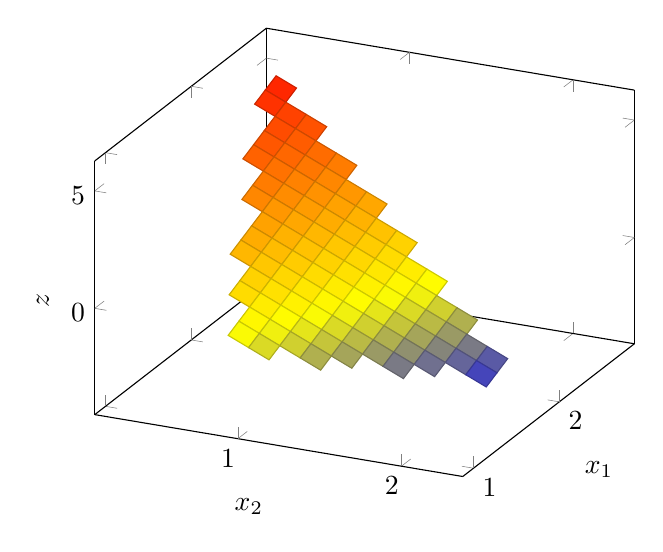
\begin{tikzpicture}
      \begin{axis}[
          xlabel=$x_2$,
          ylabel=$x_1$,
          zlabel=$z$,
          domain=0:3,
          y domain= 0:3
        ]
        \addplot3[surf, unbounded coords=jump]
        {
          2*y + x  < 6  &&
          -y + 4*x < 10 &&
          2*y + 5*x > 6  &&
          8*y - 5*x > 2  &&
          y > 0 &&
          y > 0?
          2*y-3*x:NaN
        };
      \end{axis}
    \end{tikzpicture}
    \caption{La funzione $z$}
  \end{subfigure}
  ~
  \begin{subfigure}{0.45\textwidth}
    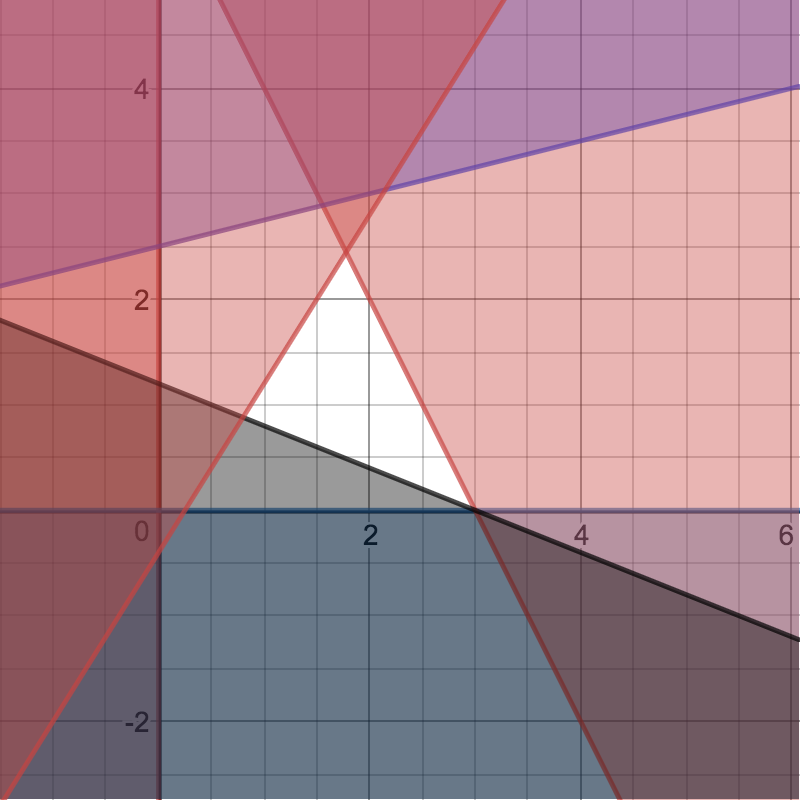
\includegraphics[width=0.8\textwidth]{2_9}
    \caption{I vincoli del problema nello spazio $x_1 - x_2$}
  \end{subfigure}
  \caption{Risoluzione esercizio 2.9}
\end{figure}

Il punto di minimo è l`angolo dove l'ordinata è massima e l'ascissa minima.

\[
  \begin{cases}
    8x_1 - 5x_2 = 2 \\
    2x_1 + x_2 = 6
  \end{cases}
  \Rightarrow
  \begin{cases}
    8x_1 - 5(6 - 2x_1) = 2 \\
    x_2 = 6 - 2x_1
  \end{cases}
  \Rightarrow
  \begin{cases}
    x_1 = \frac{16}{9} \\
    x_2 = 6 - \frac{32}{9} = \frac{54 - 32}{9}  = \frac{22}{9}
  \end{cases}
\]

Il valore di minimo della funzione risulta $\min z = \frac{32}{9} - \frac{66}{9} = \frac{34}{9}$.


\end{document}